\chapter{Neural Networks}
\label{sec:neural_networks}
In GAT-Denoiser, concepts from existing neural networks have been used.
In this chapter, GAT, Convolution and U-Net are introduced in detail.

\section{Graph Attention Networks}
The main component of GAT-Denoiser is a GAT.
GAT is an extension to GCN and adds attention (or weights) to neighbors for learning new node feature representations. 
Topology of the graph will not change but weighted averaging over the neighborhood will be computed.

\paragraph{Single Layer}
Input of a single GAT layer are node features $h = \{ h_1, h_2, \dots , h_N \} \in \mathbb{R}^F$, 
where $N$ is the number of nodes and $F$ the number of features per node. 
Single layer will map input to output, which can potentially have different dimensions: 
$h^{\prime} = \{ h_1^{\prime}, h_2^{\prime}, \dots, h_N^{\prime} \} \in \mathbb{R}^{F^{\prime}} $
As is other GNNs, input features are initially linearly transformed and parametrized by a learnable weight matrix 
$W \in \mathbb{R}^{F^{\prime} \times F}$. 
This allows to add enough expressiveness to the neural network and weights are learned during training.
Further, attention coefficients are computed, which indicates importance of node $j$ to node $i$:

\begin{equation}
  e_{ij} = a(Wh_i, Wh_j)
\end{equation}

With $a$ as the shared attentional mechanism $a : \mathbb{R}^{F^{\prime}} \times \mathbb{R}^{F^{\prime}} \mapsto \mathbb{R}$.
\citet{GAT} proposed to use a single-layer feedforward neural network, parametrized by a weight vector $a \in \mathbb{R}^{2F^{\prime}}$
and LeakyReLu as activation function.

To compare coefficients $e$ across different nodes, normalization is needed.
Therefore, softmax is used as normalization $\alpha_{ij} = softmax_j(e_{ij})$ 
such that all attention coefficient of one node sum up to 1 and therefore are nicely comparable across nodes.
Finally, new node embedding is calculated as:

\begin{equation}
  h_i^{\prime} = \sigma \left( \sum_{j \in \mathcal{N}_i} \alpha_{ij} W h_j \right)
\end{equation}

With $\sigma$ as some arbitrary activation function.

\begin{figure}[H]
  \centering
  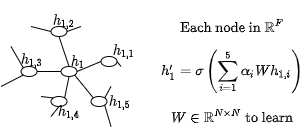
\includegraphics[width=0.6\textwidth]{GAT.drawio.png}
  \caption{GAT attention illustration example.}
  \label{fig:gat_attention_illustration}
\end{figure}


\paragraph{Multi-Head attention}
Motivated by the work of \citet{transformer}, multi-head attention can be beneficial to stabilize learning process.
Therefore, not only a single weight matrix is learned, but $W$ is split up in several parts, 
all learned individually:

\begin{equation}
  h_i^{\prime} = \bigparallel^K_{k=1} \sigma \left(\sum_{j \in \mathcal{N}_i} \alpha_{ij}^k W^k h_j \right),  
\end{equation}

Where $\parallel$ corresponds to concatenation, $\alpha_{ij}^k$ the $k$-th attention mechanism and $W^k$ the linear
transformations weight matrix. The final output consists of $KF^{\prime}$ output features.

\paragraph{Last layer:}
In the last layer, output dimension needs to be obtained. 
Consequently, concatenation is no longer plausible and averaging is used to match desired dimension.

\section{Convolution}
Convolution is an important part in Signal Processing, because it allows to average an incoming signal.
Convolution commonly operators on pixel spaces, where every observation location or time slot gets one value assigned.

\begin{equation}
  x \star k = y,
\end{equation}

Where $x$ is input signal, $k$ is kernel, $\star$ the convolution operator and $y$ the convolved signal.

To apply convolution, a kernel with weights needs to be defined. 
This kernel will then slide over the input signal $x$ and computes the dot product with its weights.
Figure~\ref{fig:1d-convolution} illustrates 1D convolution. Kernel size is set to 3, $n$ refers to input signal size and $m$ to output signal size.
In the example  $ n = m + 2$, thus, the convolved output signal size will be decreased by $2$.
The concept of convolution can be extended to arbitrary dimensions.

\begin{figure}[H]
  \centering
  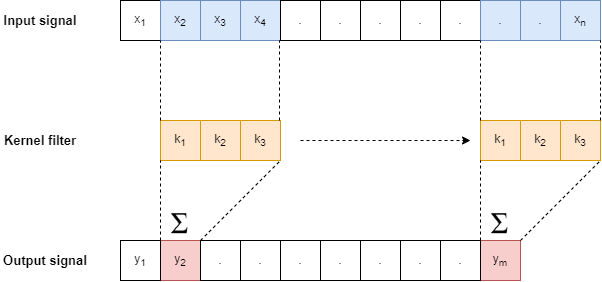
\includegraphics[width=0.6\textwidth]{Convolution.drawio.png}
  \caption{1D Convolution}
  \label{fig:1d-convolution}
\end{figure}

\paragraph{Padding:} 


Padding can be defined to add pixels to boundary of the signal.
In the example, padding is set to $0$ and therefore, the signal size is decreased by $2$.
If signal size should be fixed during convolution, padding is a powerful tool. For padding $1$,
the input size $n$ would be equal to output size $m$, as an extra element in the output signal
will be at convolved at boundaries.


\paragraph{Stride:}
Stride is the parameter how far kernel moves each time. In the example, stride was defined to be $1$.
If stride is increased, the output signal size will decrease.

\section{U-Net}
\label{sec:unet}
U-Net can boost performance of CT reconstruction, where FBP is further refined with a neural network.
It is a convolutional neural network, which is well suited for image segmentation in different domains.
\cite{unet-tomography} showed great success for biomedical image segmentation.

The neural network architecture consists of contracting path and expansive path,
resulting in a U-shape, as illustrated in Figure~\ref{fig:u-net-architectue}.

\begin{figure}[H]
  \centering
  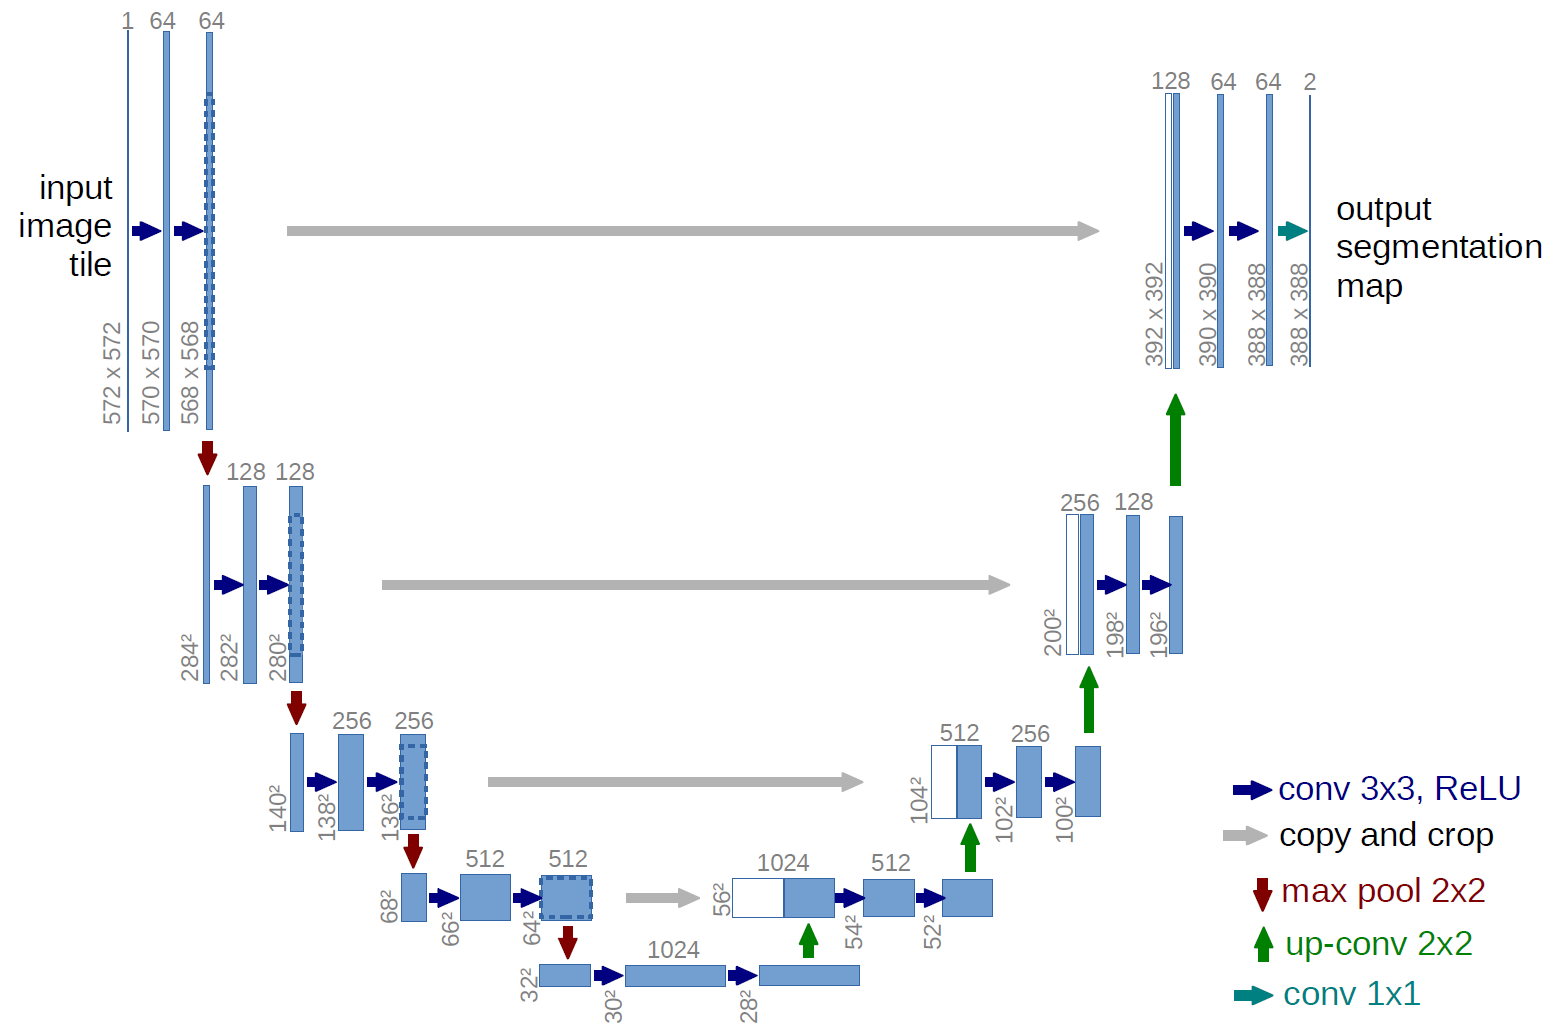
\includegraphics[width=0.6\textwidth]{u-net-architecture.png}
  \caption{
    U-Net architecture \cite[p 2, Fig. 1]{unet-tomography} \\
    Number on top of boxes denotes channels, where numbers at bottom of boxes refer to input dimension.
    }
    \label{fig:u-net-architectue}
\end{figure}


During contracting path (left part), input dimension is decreased but channels increased.
For every step in the contracting path, two 3x3 convolution layers are followed by ReLu
and a 2x2 max pooling for down-sampling. Further, at each down-sampling step, input channels are doubled.
Multiple contracting steps are combined. After last contracting step, expansive path (right part) starts
where input dimension will be increased and input channels will be decreased.
For every expansive step, an up-sampling of the feature map takes place, followed by a 2x2 convolution, 
which halves the number of channels. Then, concatenation with the corresponding feature
map of the contracting path is done (gray arrow in Figure~\ref{fig:u-net-architectue}), followed by again two 3x3 convolutions and ReLu.
Final layer is a 1x1 convolution to map to desired output dimension and single output channel.

